\documentclass{article}

\usepackage[utf8]{inputenc}
\usepackage[T1]{fontenc}
\usepackage[francais]{babel}
\usepackage{hyperref}

\hypersetup{
  unicode=false, % non-Latin characters bookmarks
  pdftoolbar=false, % show Acrobat's toolbar?
  pdfmenubar=false, % show Acrobat's menu?
  pdffitwindow=true, % page fit to window when opened
  pdfnewwindow=true, % links in new window
  pdfkeywords={polonium, P6}, % list of keywords
  colorlinks=true, % false: boxed links; true: colored links
  linkcolor=black, % color of internal links
  citecolor=green, % color of links to bibliography
  filecolor=magenta, % color of file links
  urlcolor=blue % color of external links
}

\usepackage{geometry}
\usepackage{graphicx}
\geometry{hmargin=4.0cm,vmargin=1.5cm}


\title{Rapport de conception intermédiaire\\
Projet TIA}
\author{Ronan \bsc{Abhamon}, Florian \bsc{Bigard}, Kevin \bsc{Hivert} et Nicolas \bsc{Reynaud}}
\date{2014}

\begin{document}

\maketitle

\newpage

\renewcommand{\contentsname}{Sommaire}
\tableofcontents
\newpage

\section{Description générale de l'application}

Le but de notre projet est de réaliser une interface Web permettant l'échange de vidéos au sein d'une communauté.
Le système part d'un concept simple, l'internet regorge de vidéos en tout genre, pourquoi ne pas centraliser celles digne d'intérêt ?

Il y va donc de plusieurs principes :

\paragraph{}
Cette communauté étant un ensemble de membres, nous prévoyons de créer un espace pour chaque membre. Qui dit espace dit aussi : 
compte, inscription et connexion évidemment. Ceux-ci doivent pouvoir partager des vidéos de plateformes de médias comme par exemple Youtube
(et non pas les télécharger de son ordinateur) sur notre application.
Le fait de partager n'est pas suffisant, il faut pouvoir aussi émettre une critique sur ces médias, un système de votes est donc plus
qu'envisageable. Pour renforcer ce système, la mise en place de commentaires nous semble aussi très utile. 

\paragraph{}
Ces membres doivent donc interagir sur notre application, celle-ci est constituée de 2 environnements :
\begin{itemize}
	\item Un site internet léger pour accéder aux vidéos, commentaires et autres informations.
	\item Un client lourd, soit un programme permettant d'accéder aux mêmes données que le site internet lui-même.
\end{itemize}

\paragraph{} Concernant les vidéos, elles pourront être intégrées au sein de playlists. Elles devront par ailleurs pouvoir êtres 
échangées entre les membres de cette communauté. Les vidéos n'étant rien d'autre que des urls dans notre base de données, une simple
recherche de mots clefs doit pouvoir mener à un ensemble de vidéos, une fonction recherche est donc indispensable. Enfin les utilisateurs
auront la possibilité de trier ces vidéos par date, nombre de votes ou tout autre système que nous jugerons utile.






\section{Modélisation}

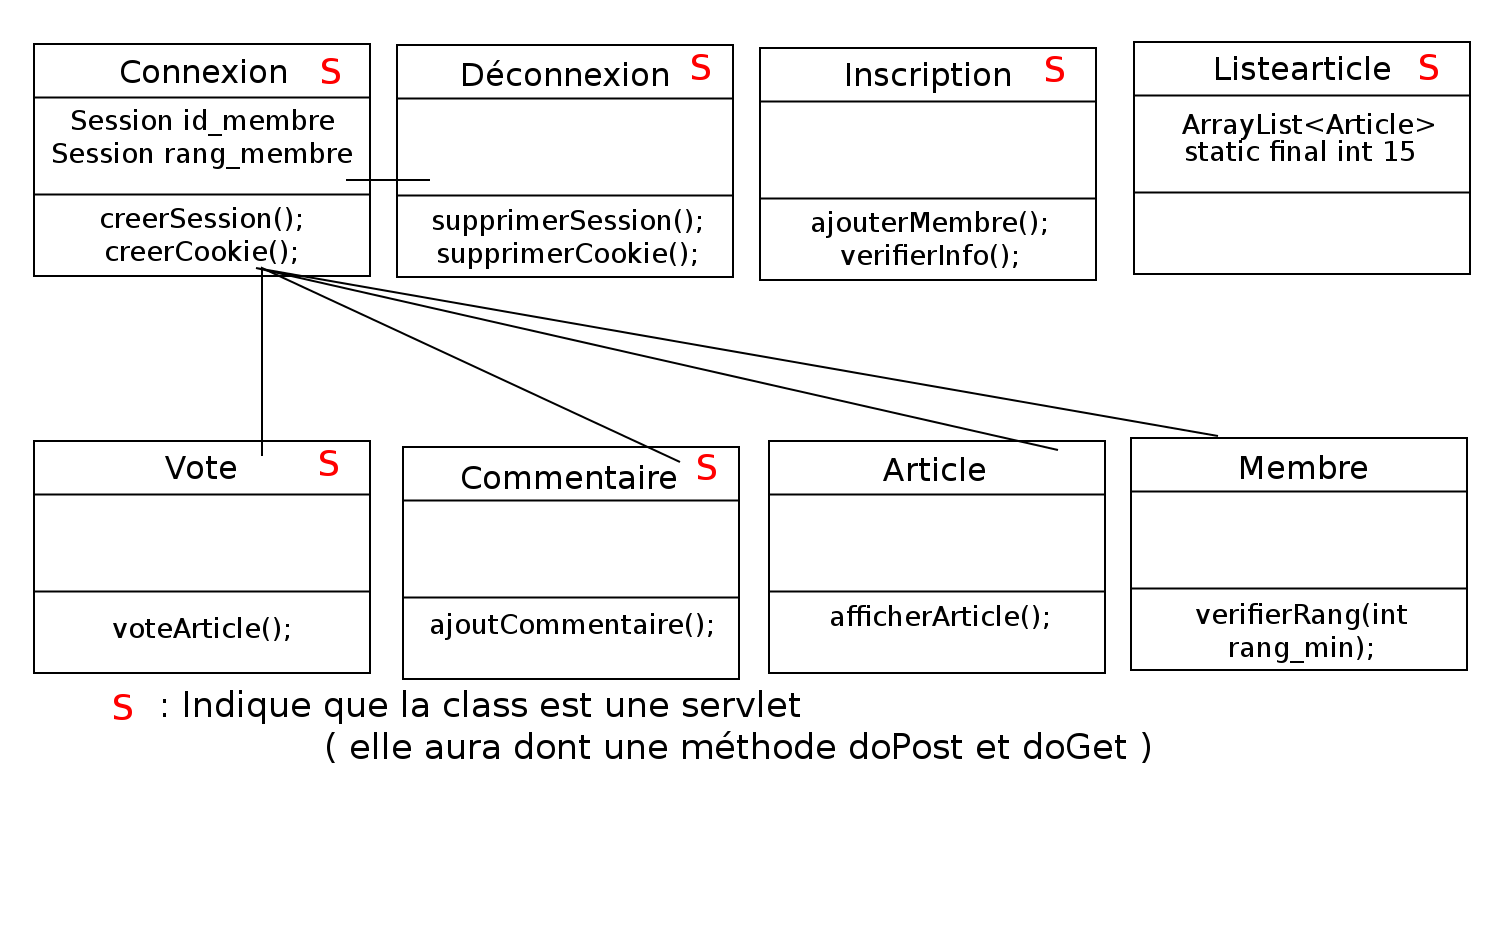
\includegraphics[scale=0.4, angle=90]{UML.png}

\newpage

\section{Plan du site}

\subsection{Pages principales}
\begin{center}
Design des pages principales
\end{center}
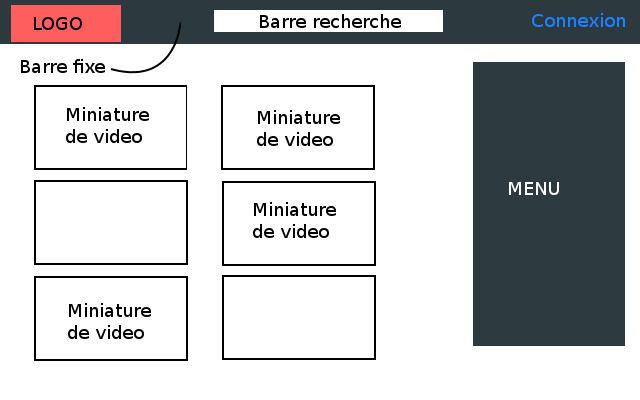
\includegraphics[scale=0.7]{design.png}


\subsubsection{Accueil}
La page accueil contiendra les miniatures des vidéos qui ont déjà été postée. Celle ci seront triée par date de publication, de la plus récente a la plus vieille.
Il s'agit de la première page visible sur le site à l’arrivée d'un visiteur.

\subsubsection{Top - Flop}
Les pages Top et Flop auront pratiquement la même fonction que la page accueil, cependant la page Top triera les vidéos par nombre de vote croissant [ des plus appréciées aux moins appréciées ]. Et la page Flop dans le nombre décroissant de votes [ Des moins appréciées aux plus appréciées ].
\newpage
\subsection{Pages associées a une vidéo}
\begin{center}
Design des pages d'affichage de vidéos
\end{center}
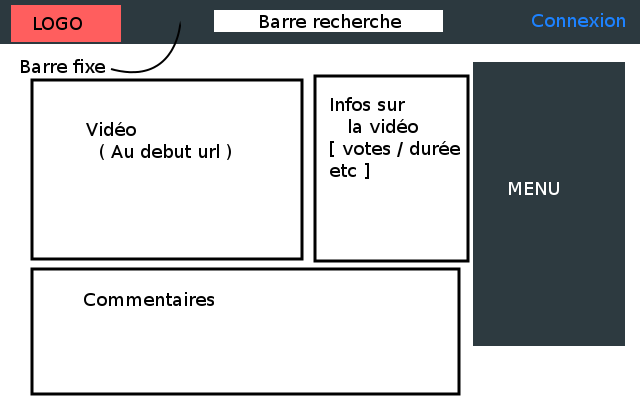
\includegraphics[scale=0.7]{pages.png}

\subsubsection{Visualisation d'une vidéo}

\subsubsection{Random}
La page random donnera une vidéo de façon aléatoire parmi toutes celles disponible sur le site.
\newpage
\subsection{Pages secondaires - Formulaires}
\begin{center}
Design des pages secondaires
\end{center}
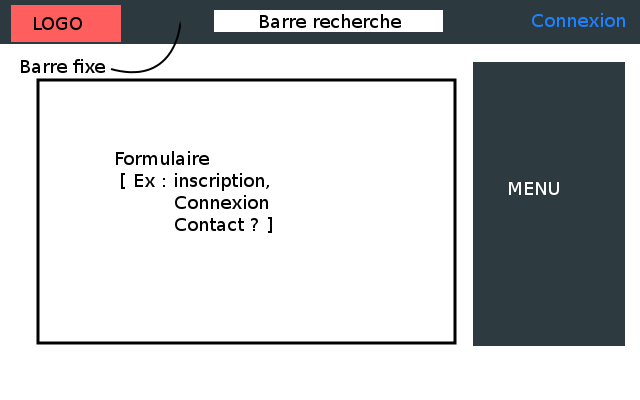
\includegraphics[scale=0.7]{formulaires.png}


En adaptant la taille du cadre formulaire bien entendu
\subsubsection{Inscription}
Cette page permettra a un visiteur de s'inscrire pour qu'il devienne membre de la communauté.

\subsubsection{Connexion}
La page connexion permettra aux membres du site de se connecter passant leurs status de visiteur a membres.

\subsubsection{Déconnexion}
La page déconnexion aura pour but de déconnecter une personne si elle est connectée.

\subsubsection{Poster article}
Cette page permettra simplement aux membres de poster un article.

\newpage
\section{Utilisation des technologies}

\subsection{HTML5/CSS3}
Le client léger étant un navigateur Web, il faut que notre serveur affiche des pages Web, et donc HTML. Nous avons choisi de combiner HTML5 et CSS3 afin de profiter des dernières avancées dans le secteur du Web et ainsi empêcher les utilisateurs d'Internet Explorer d'accéder à notre site. De plus, à terme nous prévoyons d'afficher directement les vidéos (au lieu de juste un lien YouTube), il sera donc intéressant d'exploiter la balise \emph{video} d'HTML5.

\subsection{JavaScript/JQuery}
Nous pensons aussi exploiter le JavaScript et notamment le JQuery afin de rendre le site plus dynamique (votes en AJAX par exemple), avec pourquoi pas quelques animations. Encore une fois, si nous voulons afficher nous-même les vidéos il sera intéressant d'exploiter le JavaScript. Quant au JQuery, il nous permettrait un développement plus rapide (cette partie n'étant pas essentielle, il ne serait pas judicieux d'y passer trop de temps).

\subsection{Java/Servlet}
Bien évidemment, nous devrons utiliser les Servlets et Java afin de générer nos pages Web. Tout le moteur de notre serveur Web sera donc réalisé en Java.

\subsection{SQL}
Toutes les données concernant les membres, les vidéos, les votes, commentaires... seront stockés dans une base de données SQL. Java communiquera donc avec la base de données avec les pilotes adaptés (JDBC). Il créera les objets grâce aux données récupérées de la base SQL, qu'il pourra ainsi afficher, modifier ou supprimer. Bien évidemment, il pourra aussi insérer de nouvelles données.

\subsection{XML}
L'utilisateur peut exporter une liste de vidéos au format XML (une playlist par exemple) et ainsi la sauvegarder pour la réimporter plus tard. Un membre pourra aussi facilement envoyer une playlist à autre membre. En effet, la playlist étant du XML (et donc au format texte), elle pourra facilement s'envoyer (que ce soit via une base de données, ou tout simplement via des sockets).

\subsection{Java/Swing}
Le client lourd sera réalisé en Java à l'aide de la bibliothèque Swing. Cette application reprendra grosso-modo le même design que le site web.

\subsection{Sockets TCP}
En ce qui concerne le tchat P2P entre deux clients lourds, nous utiliserons simplement les sockets TCP. 

\newpage
\section{Répartition du travail et désignation d'un chef}
\subsection{Chef d'équipe}
Notre chef d'équipe sera : Nicolas REYNAUD

\subsection{Répartition du travail}

\begin{description}
  \item[Swing] \textbf{Ronan} s'occupera de l'aspect visuel du client lourd à l'aide de swing, et également du design global du site.
  \item[Servlet] \textbf{Nicolas \& Kevin} s’occuperont de la partie Web avec notamment les servlets. Nicolas s'occupera en plus de la Base de donnée.
  \item[Tchat] \textbf{Florian} s'occupera de la partie du tchat en Peer to Peer ( P2P ), ainsi que du client lourd avec Ronan.
\end{description}

\end{document} 

